\documentclass[conference]{IEEEtran}

\usepackage[T1]{fontenc}
\usepackage[utf8]{inputenc}
\usepackage{amsmath}
\usepackage{amssymb}
\usepackage{booktabs}
\usepackage{array}
\usepackage{url}
\usepackage{listings}
\usepackage{xcolor}
\usepackage{graphicx}
\usepackage{fancyhdr}
\usepackage{tikz}
\usepackage{pgfplots}
\pgfplotsset{compat=1.18}
\usepgfplotslibrary{fillbetween}
\usetikzlibrary{arrows.meta,positioning,shapes.geometric,calc}
\graphicspath{{figures/}{docs/figures/}}
\renewcommand\IEEEkeywordsname{Keywords}

\lstdefinestyle{terminalstyle}{
  basicstyle=\ttfamily\footnotesize,
  breaklines=true,
  columns=fullflexible,
  frame=single,
  backgroundcolor=\color{gray!8}
}
\lstset{style=terminalstyle}

\tikzset{
  block/.style={draw, rounded corners, align=center, font=\footnotesize,
    minimum height=8mm, text width=25mm},
  wideblock/.style={draw, rounded corners, align=center, font=\footnotesize,
    minimum height=8mm, text width=34mm},
  smallblock/.style={draw, rounded corners, align=center, font=\scriptsize,
    minimum height=7mm, text width=20mm},
  arrow/.style={-Latex, thick}
}

\begin{document}

\pagestyle{fancy}
\fancyhf{}
\fancyhead[L]{\scriptsize F.Y.B. Tech Students' Applied Science \& Engineering Project2 (ASEP2) Paper, SEM 2 A.Y. 2025-26 \quad Vishwakarma Institute of Technology, Pune, INDIA.}
\fancyhead[R]{\scriptsize \thepage}
\renewcommand{\headrulewidth}{0pt}
\setlength{\headheight}{13.6pt}

\title{A Real-Time Multi-Engine Research Terminal for Precious-Metal Market Intelligence}

\author{
\IEEEauthorblockN{Ramakrishna Bharsakde, Parth Dongre, Parth Birari, Atharv Patil, Aryan Patil}
\IEEEauthorblockA{
Department of Engineering, Sciences and Humanities (DESH)\\
Vishwakarma Institute of Technology, Pune, Maharashtra, India}
}

\maketitle
\thispagestyle{fancy}

\begin{abstract}
Precious-metal markets are shaped by interactions among monetary policy,
inflation expectations, real interest rates, currency strength, liquidity,
cross-asset risk sentiment, and short-horizon order-flow pressure. A research
terminal for such markets must therefore evaluate price action through
multiple complementary lenses rather than relying on a single technical
indicator or isolated chart. This paper presents Metals Terminal, a local
research terminal for gold and silver market intelligence centered on the
\texttt{XAUUSDT} and \texttt{XAGUSDT} instruments. The system integrates a
FastAPI and WebSocket backend, a browser-based analytical frontend, a
registry of 71 quantitative engines, telemetry logging, Monte Carlo
simulation, technical indicator overlays, live order-book microstructure,
replay scorecards, macro overlays, offline demonstration mode, and native C++
acceleration. The architecture is designed for undergraduate research-scale
deployment: transparent, reproducible, inexpensive to operate, and
packageable as a desktop application. The paper formalizes the market
analysis process used by the terminal, including trend confirmation,
momentum exhaustion, volatility expansion, volume participation,
microstructure pressure, cross-asset confirmation, and scenario-based risk
assessment. Evaluation focuses on system correctness, JSON-safe snapshot
contracts, memory-aware tick storage, bundle-build efficiency, backtest
replay, interface completeness, and desktop packaging. Test results show that
the implemented suite passes 38 automated tests, while the packaging workflow
produces a verified desktop artifact. The work demonstrates that a modular
multi-engine financial research terminal can be implemented with open-source
tools while preserving interpretability, computational discipline, and
research reproducibility.
\end{abstract}

\begin{IEEEkeywords}
Financial technology, market microstructure, technical analysis, real-time
systems, FastAPI, WebSocket, Monte Carlo simulation, precious metals, software
engineering, desktop packaging.
\end{IEEEkeywords}

\section{Introduction}

Gold and silver are widely studied assets because they respond to monetary
conditions, inflation expectations, currency strength, industrial demand,
safe-haven demand, liquidity stress, and broader risk sentiment. Gold often
behaves as a macro-sensitive store-of-value asset, while silver combines
precious-metal behavior with greater sensitivity to industrial demand and
cyclical growth expectations. In both markets, short-term price behavior is
frequently determined by the interaction between higher-timeframe
macroeconomic forces and lower-timeframe microstructure conditions such as
spread, depth, and order-book imbalance.

Market participants therefore examine a broad set of signals: moving
averages, volatility bands, relative strength, momentum divergence,
order-book imbalance, realized volatility, support and resistance, regime
shifts, cross-asset relationships, and probabilistic risk estimates. A
frequent limitation of lightweight academic or educational market terminals
is that they display these components as independent charts. Such a
presentation can be visually useful, but it does not by itself provide a
reproducible analytical process. A research-oriented terminal must instead
connect data ingestion, feature computation, signal normalization,
explainable visualization, telemetry, and verification into a single
auditable workflow.

The objective of Metals Terminal is to build a local research system that
answers a practical question: can an undergraduate engineering project
combine real-time data ingestion, market microstructure features, classical
technical indicators, statistical regime analysis, interpretable
visualizations, backtest-oriented validation, and desktop packaging without
relying on external compute infrastructure?

The project is not designed to provide financial advice or automated trade
execution. Instead, it focuses on research instrumentation: capturing data,
computing explainable features, scoring independent engines, visualizing
state, and preserving enough telemetry for later review. The system is
implemented as a Python package named \texttt{metals}, with a FastAPI server
and a vanilla JavaScript frontend served locally. The implementation contains
71 registered engines, live WebSocket feeds, a technical indicator manager
with 25 toggles, Monte Carlo simulation controls, chart panels, telemetry
exports, and platform-specific desktop packaging scripts.

The main contributions of this project are:
\begin{enumerate}
  \item A modular real-time market research architecture for gold and silver.
  \item A 71-engine registry spanning trend, momentum, volatility, risk,
  microstructure, regime, spectral, cross-asset, macro, and forecasting
  families.
  \item A formal market-analysis workflow that combines directional bias,
  confirmation, volatility/risk control, and execution-context inspection.
  \item A JSON-safe snapshot protocol for streaming engine outputs to a
  frontend.
  \item A responsive terminal interface with engine visualizations, chart
  indicators, Monte Carlo simulation, currency controls, and time controls.
  \item Memory-efficiency improvements for tick storage, slow-engine cadence,
  and frontend rendering.
  \item A completed enhancement layer containing live depth-based
  microstructure, replay validation, macro overlays, offline demonstration
  mode, and signed desktop packaging workflows.
\end{enumerate}

\section{Related Work}

Financial research terminals commonly combine market data, indicators, risk
analytics, and order-book views. Professional systems such as Bloomberg
Terminal and Refinitiv Workspace provide broad data coverage and execution
workflows, but their complexity and cost are not suitable for small academic
projects. Open-source charting and backtesting frameworks are more accessible
but usually require developers to assemble ingestion, analytics, serving, and
visualization components manually.

Technical analysis literature provides the first layer of the system.
Wilder introduced several widely used momentum and volatility measures,
including RSI, ATR, and directional movement concepts \cite{wilder1978}.
Bollinger Bands provide a volatility-normalized envelope around a moving
average and remain useful for visualizing expansion, compression, and
mean-reversion zones \cite{bollinger2001}. Metals Terminal implements these
classical indicators as chart overlays and oscillator panes so the user can
connect engine scores to familiar market tools.

Financial time-series research contributes the second layer. Hamilton's
regime-switching view and Tsay's treatment of financial return dynamics
support the use of volatility states, autocorrelation checks, and
distribution-aware validation \cite{hamilton1994,tsay2010}. Lopez de Prado's
work motivates careful walk-forward validation, feature leakage control, and
probabilistic interpretation rather than raw in-sample performance claims
\cite{lopez2018}. For this reason, the paper reports software verification
and replay-oriented out-of-sample metrics instead of claiming trading
profitability.

Market microstructure research forms the third layer. Order-flow imbalance,
liquidity, and flow toxicity are used to understand whether short-term price
movement is supported by depth or pressure. Easley, Lopez de Prado, and
O'Hara introduced VPIN-style flow toxicity as a way to reason about adverse
selection in high-frequency markets \cite{easley2012}. Kyle's lambda and
Amihud illiquidity proxies measure price impact per unit of signed or total
volume. Metals Terminal uses simplified educational versions of these ideas
because full exchange-grade microstructure modeling would require richer
trade classification and depth history.

Cross-asset and spectral research adds broader context. Diebold and Yilmaz
show that spillover concepts can quantify directional relationships between
markets \cite{diebold2012}. Mallat's wavelet framework supports localized
time-frequency analysis, which is useful when market cycles are nonstationary
\cite{mallat1989}. These ideas motivate the project's cross-asset,
lead-lag, spectral, wavelet, and complexity engines.

From a software-engineering perspective, FastAPI provides typed HTTP and
WebSocket services, PyInstaller provides desktop packaging, and Lightweight
Charts provides responsive browser rendering \cite{fastapi,pyinstaller,
lightweightcharts}. Binance USD-M futures endpoints supply the public market
data used by the prototype \cite{binance}. The gap addressed by this project
is the integration of these separate concepts into one local, explainable,
undergraduate research-scale terminal with tests, memory controls, diagrams,
simulation, and packaging.

\section{Market Analysis Framework}

The analytical foundation of Metals Terminal is that no single indicator is
sufficient to describe the state of a precious-metal market. A moving average
may identify trend direction but cannot measure liquidity risk. RSI may
identify momentum exhaustion but does not quantify the magnitude of a
potential adverse move. Order-book imbalance may describe immediate pressure
but can become noisy without higher-timeframe context. The terminal therefore
uses a layered market-analysis framework in which independent evidence
families are computed, normalized, visualized, and interpreted together.

\subsection{Precious-Metal Market Drivers}

Gold and silver prices are influenced by both macroeconomic variables and
market-internal variables. The macroeconomic layer includes real yields,
nominal interest-rate expectations, inflation expectations, central-bank
policy, dollar strength, geopolitical risk, and broad risk appetite. Higher
real yields generally increase the opportunity cost of holding non-yielding
assets such as gold, while weaker real yields and inflation uncertainty often
increase demand for precious metals. The currency layer is also important
because gold and silver are typically quoted in U.S. dollars; dollar strength
can pressure dollar-denominated metal prices even when local-currency demand
remains stable.

The market-internal layer includes price trend, realized volatility, volume
participation, support and resistance behavior, order-book depth, spread, and
short-horizon flow pressure. These variables help distinguish a strong
directional move from a thin-liquidity movement. For example, a gold breakout
accompanied by rising volume, narrow spread, positive order-book pressure,
and favorable cross-asset confirmation is analytically stronger than a
breakout occurring with weak volume and unstable liquidity.

\begin{table*}[!t]
\caption{Market Variables Used in Precious-Metal Analysis}
\label{tab:market-drivers}
\centering
\begin{tabular}{@{}p{0.18\textwidth}p{0.34\textwidth}p{0.38\textwidth}@{}}
\toprule
\textbf{Driver} & \textbf{Market Interpretation} & \textbf{Terminal Measures} \\
\midrule
Trend structure & Directional persistence and breakout quality &
Moving averages, Supertrend, Ichimoku, ADX \\
Momentum & Speed of movement and exhaustion risk &
RSI, MACD, stochastic, ROC, divergence \\
Volatility & Risk, range expansion, stop distance &
ATR, realized volatility, Bollinger width, VaR \\
Volume and flow & Participation behind price movement &
VWAP, OBV, volume SMA, CVD-style flow \\
Microstructure & Immediate liquidity and pressure &
Spread, depth, imbalance, microprice, VPIN proxy \\
Cross-asset context & Confirmation across related markets &
Gold-silver ratio, beta, lead-lag, CoVaR \\
Macro context & Monetary and sentiment environment &
Real-yield proxy, curve structure, news sentiment \\
\bottomrule
\end{tabular}
\end{table*}

\subsection{Analytical Questions}

The terminal is designed around five recurring market-analysis questions:
\begin{enumerate}
  \item \textit{Direction:} is the market trending, ranging, or reversing?
  \item \textit{Participation:} is the movement confirmed by volume and flow?
  \item \textit{Volatility:} is the current range expanding, compressing, or
  entering a tail-risk state?
  \item \textit{Liquidity:} can the observed price movement be supported by
  available depth and spread conditions?
  \item \textit{Scenario risk:} how sensitive is the market hypothesis to
  volatility shocks, liquidity shocks, and adverse price paths?
\end{enumerate}

This structure prevents the system from treating a single bullish or bearish
indicator as sufficient evidence. Instead, each market state is interpreted
through a combination of directional, risk, and liquidity evidence. This is
especially relevant for gold and silver because these instruments can
transition quickly between macro-driven trending regimes and short-term
liquidity-driven reversals.

\subsection{Indicator Confirmation Philosophy}

Technical indicators are most useful when interpreted as measurements of
different market properties rather than as independent trading rules. Moving
averages and Ichimoku-style components describe trend and structural support.
RSI, stochastic oscillators, and MACD describe momentum and acceleration.
Bollinger Bands, ATR, and realized volatility describe range and risk. VWAP,
OBV, and volume measures describe participation. Order-book metrics describe
immediate execution context. Metals Terminal groups indicators by these
analytical roles and then displays both the raw visual state and the
normalized engine score, enabling a user to compare classical chart evidence
with quantitative engine evidence.

\section{System Requirements}

The requirements were selected for an undergraduate engineering research
project in which reproducible system behavior, market explainability, and
software verification are as important as model complexity.

\subsection{Functional Requirements}

The system must fetch historical gold and silver market data, subscribe to
live tick and order-book updates, compute multiple families of indicators and
engines, fuse engine scores into a master signal, stream snapshots to a
frontend without JSON serialization failures, render charts and risk panels,
allow symbol/timeframe/currency/layout/simulation controls, store telemetry,
run locally, and be packageable as a desktop application.

\subsection{Non-Functional Requirements}

The system must remain usable in a local development environment, avoid unbounded memory growth from
tick data, defer expensive engines when appropriate, keep frontend panels
responsive, use testable module boundaries, degrade gracefully when optional
macro/news/COT data is unavailable, and preserve transparent outputs instead
of opaque predictions.

\section{Architecture}

The project is organized as a Python package and browser frontend. The
high-level module structure is:

\begin{lstlisting}
metals/
  config.py        configuration and paths
  contracts.py     Tick, EngineResult, Bundle contracts
  orchestrator.py  engine execution and bundle construction
  data/            REST, WebSocket, cache, order-book data
  engines/         registered analysis engines
  serve/           FastAPI routes, WebSockets, snapshots
  web/             HTML, CSS, JavaScript terminal UI
  backtest/        replay, walk-forward, scorecard, DSL
  ml/              feature store, ensemble, calibration
mtxcore/           optional C++ acceleration kernels
tests/             unit and contract tests
packaging/         PyInstaller specification
scripts/           desktop build scripts
\end{lstlisting}

Fig.~\ref{fig:architecture} describes the high-level data flow.

\begin{figure*}[!t]
\centering
\resizebox{0.98\textwidth}{!}{%
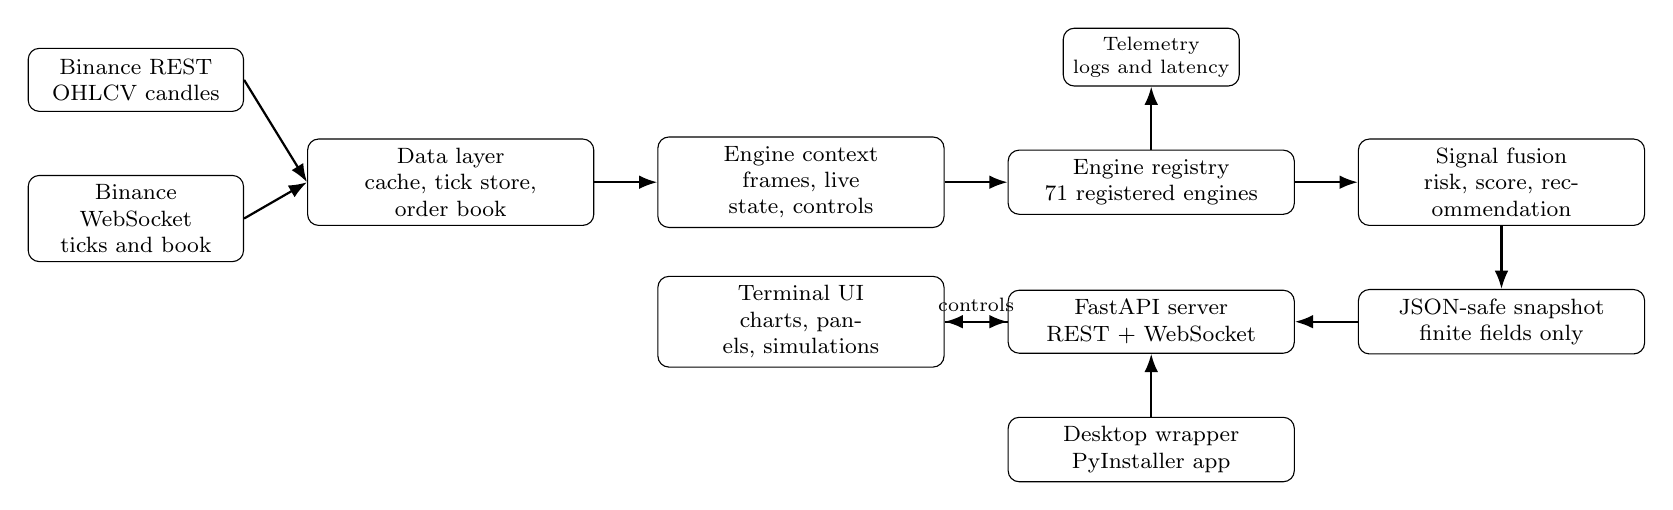
\begin{tikzpicture}[node distance=8mm and 8mm]
  \node[block] (rest) {Binance REST\\OHLCV candles};
  \node[block, below=of rest] (ws) {Binance WebSocket\\ticks and book};
  \node[wideblock, right=of rest, yshift=-13mm] (data) {Data layer\\cache, tick store, order book};
  \node[wideblock, right=of data] (context) {Engine context\\frames, live state, controls};
  \node[wideblock, right=of context] (registry) {Engine registry\\71 registered engines};
  \node[wideblock, right=of registry] (fusion) {Signal fusion\\risk, score, recommendation};
  \node[wideblock, below=of fusion] (snapshot) {JSON-safe snapshot\\finite fields only};
  \node[wideblock, left=of snapshot] (server) {FastAPI server\\REST + WebSocket};
  \node[wideblock, left=of server] (frontend) {Terminal UI\\charts, panels, simulations};
  \node[wideblock, below=of server] (desktop) {Desktop wrapper\\PyInstaller app};
  \node[smallblock, above=of registry] (telemetry) {Telemetry\\logs and latency};

  \draw[arrow] (rest.east) -- (data.west);
  \draw[arrow] (ws.east) -- (data.west);
  \draw[arrow] (data) -- (context);
  \draw[arrow] (context) -- (registry);
  \draw[arrow] (registry) -- (fusion);
  \draw[arrow] (fusion) -- (snapshot);
  \draw[arrow] (snapshot) -- (server);
  \draw[arrow] (server) -- (frontend);
  \draw[arrow] (frontend) -- node[font=\scriptsize, above]{controls} (server);
  \draw[arrow] (desktop) -- (server);
  \draw[arrow] (registry) -- (telemetry);
\end{tikzpicture}}
\caption{Block diagram of the Metals Terminal real-time research architecture.}
\label{fig:architecture}
\end{figure*}

\begin{figure*}[!t]
\centering
\includegraphics[width=0.92\textwidth]{metals-terminal-landing.png}
\caption{Project screenshot of the Metals Terminal landing view showing live
gold and silver status, master score, build latency, tick rate, and dashboard
navigation.}
\label{fig:screenshot-landing}
\end{figure*}

The backend has two primary real-time channels. The \texttt{/ws} endpoint
streams bundle snapshots containing candles, engine outputs, signal state,
risk metrics, and visualization payloads. The \texttt{/ws/live} endpoint
streams fast live ticks containing latest price, order-book summary, spreads,
book pressure, and live alert events. The frontend is intentionally
implemented with vanilla JavaScript and lightweight browser libraries to keep
the project understandable and reduce build-tool complexity.

\begin{table}[!t]
\caption{Primary Runtime Interfaces}
\label{tab:interfaces}
\centering
\begin{tabular}{@{}p{0.25\linewidth}p{0.22\linewidth}p{0.43\linewidth}@{}}
\toprule
\textbf{Interface} & \textbf{Type} & \textbf{Role} \\
\midrule
\texttt{/} & HTTP & Serves the terminal frontend \\
\texttt{/api/snapshot} & HTTP & Returns one bundle snapshot for polling/debugging \\
\texttt{/ws} & WebSocket & Streams slower analytical bundles \\
\texttt{/ws/live} & WebSocket & Streams fast tick and order-book updates \\
\texttt{/api/simulate} & HTTP & Runs bounded Monte Carlo scenarios \\
\texttt{/health} & HTTP & Confirms backend readiness for launcher \\
\bottomrule
\end{tabular}
\end{table}

\subsection{Snapshot Contract}

The backend converts a bundle $B_t$ into a frontend snapshot
\begin{equation}
\Omega_t = f_{\mathrm{snap}}(B_t),
\end{equation}
where $f_{\mathrm{snap}}$ removes non-finite values and converts arrays,
NumPy scalars, timestamps, and engine payloads into JSON-safe fields. The
contract is:
\begin{equation}
\forall x\in\Omega_t,\quad x\notin\{\mathrm{NaN},+\infty,-\infty\}.
\end{equation}
This invariant is important because one invalid numeric value can break a
browser chart or WebSocket client. Snapshot contract tests therefore check
that all streamed values are serializable and finite.

\subsection{Frontend State Model}

The frontend maintains state
\begin{equation}
\mathcal{U}_t=(\text{symbol},\text{timeframe},\text{currency},\text{layout},
\text{active indicators}).
\end{equation}
Changing symbol, timeframe, or currency increments a generation counter so
stale WebSocket messages from an earlier subscription are ignored. If
$g(m)\neq g_{current}$ for an incoming message $m$, the renderer discards it.
This prevents gold and silver views from briefly overwriting each other when
the user switches instruments.

\section{Methodology and Experimental Design}

The project methodology follows an engineering research cycle similar to the
ASEP2 project structure: define the analytical problem, design a modular
architecture, implement independent components, verify contracts through
tests, and package the final system for demonstration. The experimental unit
is not a single predictive model; it is a complete real-time pipeline that
must ingest data, compute features, fuse signals, render visualizations, and
remain stable under user interaction.

\subsection{Input and Output Definition}

The input set is
\begin{equation}
\mathcal{I}_t=\{X_{1:t}^{gold},X_{1:t}^{silver},L_t,U_t\},
\end{equation}
where $X_{1:t}$ denotes historical candles, $L_t$ denotes the latest live
book/tick state, and $U_t$ denotes user controls such as timeframe, currency,
symbol, active indicators, and simulation settings. The output set is
\begin{equation}
\mathcal{O}_t=\{\Omega_t,\Gamma_t,\Pi_t,\Sigma_t\},
\end{equation}
where $\Omega_t$ is the streamed bundle snapshot, $\Gamma_t$ is the chart
state, $\Pi_t$ is the panel visualization state, and $\Sigma_t$ is the
simulation response.

\subsection{Market-Analysis Workflow}

The analytical workflow follows a top-down structure. First, the system
estimates directional bias from trend and regime engines. This includes
moving-average alignment, trend quality, multi-timeframe slope, and
state-transition measures. Second, the system evaluates whether momentum
confirms or contradicts the trend. RSI, MACD, stochastic oscillators, rate of
change, and divergence engines are used to identify continuation,
deceleration, or exhaustion. Third, the system measures volatility and risk
through ATR, realized volatility, tail-risk measures, jump detection, and
value-at-risk estimates. Fourth, the system examines participation and
liquidity through volume indicators, VWAP, order-book imbalance, spread,
depth, and microprice. Finally, cross-asset and macro engines compare the
primary metal with related instruments and broader risk variables.

The result is not a binary rule such as ``buy when RSI is below 30.'' Instead,
the system computes a structured evidence set:
\begin{equation}
\mathcal{E}_t =
\{\mathcal{T}_t,\mathcal{M}_t,\mathcal{V}_t,\mathcal{L}_t,\mathcal{C}_t\},
\end{equation}
where $\mathcal{T}_t$ is trend evidence, $\mathcal{M}_t$ is momentum
evidence, $\mathcal{V}_t$ is volatility and risk evidence, $\mathcal{L}_t$ is
liquidity and participation evidence, and $\mathcal{C}_t$ is cross-asset and
macro context. The master signal is a summary of this evidence set, while
the terminal panels preserve the individual components so that the user can
inspect whether the final recommendation is supported by coherent evidence
or driven by only a small subset of engines.

\subsection{Program Flow}

The runtime flow is shown in Fig.~\ref{fig:program-flow}. A desktop launcher
starts the backend, waits for a health check, opens the terminal UI, and then
maintains two live paths: a slow analytical bundle path and a fast tick path.
This separation is important because chart and price-strip updates should
remain responsive even when slower engines are deferred.

\begin{figure*}[!t]
\centering
\resizebox{0.82\textwidth}{!}{%
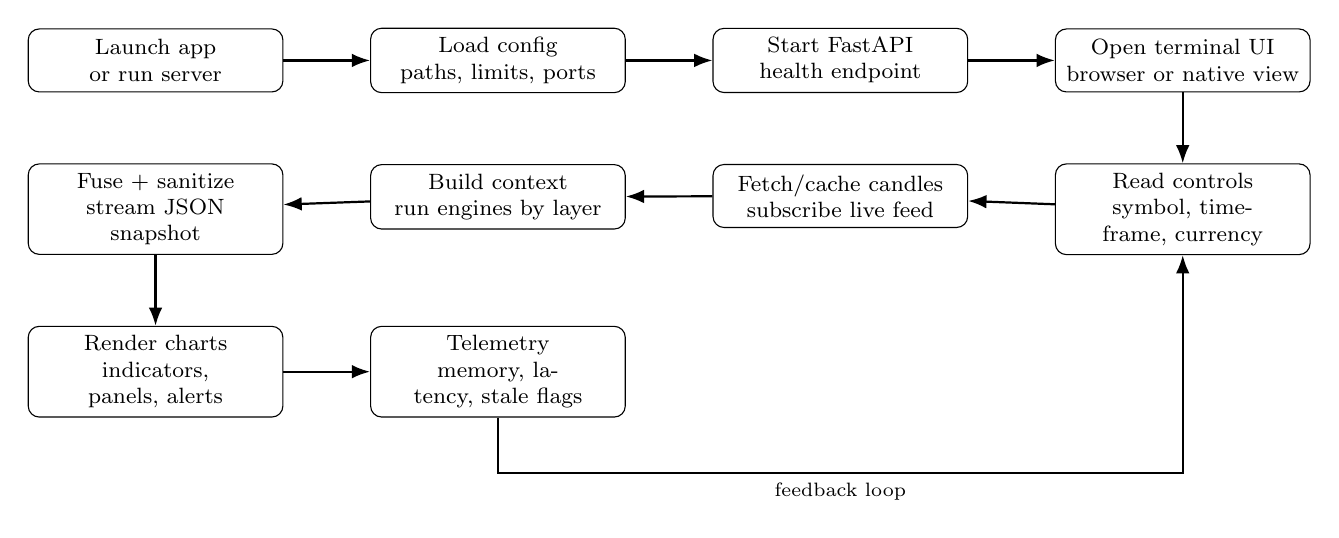
\begin{tikzpicture}[
  node distance=9mm and 11mm,
  flowblock/.style={draw, rounded corners, align=center, font=\footnotesize,
    minimum height=8mm, text width=30mm}
]
  \node[flowblock] (launch) {Launch app\\or run server};
  \node[flowblock, right=of launch] (config) {Load config\\paths, limits, ports};
  \node[flowblock, right=of config] (server) {Start FastAPI\\health endpoint};
  \node[flowblock, right=of server] (ui) {Open terminal UI\\browser or native view};

  \node[flowblock, below=of ui] (controls) {Read controls\\symbol, timeframe, currency};
  \node[flowblock, below=of server] (fetch) {Fetch/cache candles\\subscribe live feed};
  \node[flowblock, below=of config] (engines) {Build context\\run engines by layer};
  \node[flowblock, below=of launch] (snapshot) {Fuse + sanitize\\stream JSON snapshot};

  \node[flowblock, below=of snapshot] (charts) {Render charts\\indicators, panels, alerts};
  \node[flowblock, right=of charts] (telemetry) {Telemetry\\memory, latency, stale flags};

  \draw[arrow] (launch) -- (config);
  \draw[arrow] (config) -- (server);
  \draw[arrow] (server) -- (ui);
  \draw[arrow] (ui) -- (controls);
  \draw[arrow] (controls) -- (fetch);
  \draw[arrow] (fetch) -- (engines);
  \draw[arrow] (engines) -- (snapshot);
  \draw[arrow] (snapshot) -- (charts);
  \draw[arrow] (charts) -- (telemetry);
  \draw[arrow] (telemetry.south) -- ++(0,-7mm) -|
    node[font=\scriptsize, near start, below]{feedback loop} (controls.south);
\end{tikzpicture}}
\caption{Program flow from launch to live rendering and telemetry feedback.}
\label{fig:program-flow}
\end{figure*}

\begin{figure*}[!t]
\centering
\includegraphics[width=0.92\textwidth]{metals-terminal-live.png}
\caption{Project screenshot of the live terminal view with interactive
controls, market state, chart area, indicator tables, and real-time analytical
panels.}
\label{fig:screenshot-live}
\end{figure*}

\subsection{Live Pipeline Algorithm}

\begin{lstlisting}[caption={Live bundle construction and rendering pipeline.},label={alg:live-pipeline}]
Input: symbol, peer, timeframe, currency, indicators
Output: JSON-safe terminal snapshot

1. Resolve selected symbol and peer instrument.
2. Load historical OHLCV frame from cache or REST.
3. Read latest live tick and order-book state.
4. Convert currency for display-only price fields.
5. Construct EngineContext from candles and live state.
6. For each dependency layer:
      a. Reuse cached slow-engine result when valid.
      b. Execute active engines within time budget.
      c. Mark deferred outputs as stale.
7. Normalize engine scores to [0, 100].
8. Fuse weighted scores into master recommendation.
9. Compute risk, regime, forecast, and visualization payloads.
10. Replace NaN and infinite values with safe null/scalars.
11. Send snapshot over /ws and ticks over /ws/live.
12. Render charts, toggled indicators, panels, and alerts.
\end{lstlisting}

\subsection{Testing Strategy}

The testing strategy is contract driven. Engine tests verify registration,
score range, and minimal payload structure. Snapshot tests verify that
frontend payloads contain finite JSON-safe values. Tick-store tests verify
bounded queues and chunked persistence. Orchestrator tests verify slow-engine
deferral and stale flags. API tests verify Monte Carlo input limits and
response shape. Frontend asset tests verify that the required controls,
indicator toggles, and visualization panels exist in the static files.

\section{Data Layer}

The default live data source is Binance USD-M futures data for
\texttt{XAUUSDT} and \texttt{XAGUSDT}. The data layer is divided into
historical REST retrieval, live WebSocket streaming, order-book state, and
local cache management.

\subsection{Historical Data}

Historical OHLCV candles are fetched through Binance REST endpoints and
cached locally. This reduces repeated network calls and provides stable input
frames for engines. The system supports multiple timeframes, including
1-minute, 5-minute, 15-minute, 30-minute, 1-hour, 2-hour, 4-hour, 6-hour,
12-hour, and daily bars.

\subsection{Live Data}

The live WebSocket path receives market ticks and order-book updates. These
updates are used by the frontend live strip and by microstructure engines.
The live channel is separated from the heavier bundle channel so fast price
updates do not require full engine recomputation.

\subsection{Tick Storage}

Earlier designs can accidentally grow memory by accumulating ticks in memory
or rewriting large daily files repeatedly. Metals Terminal uses bounded tick
queues and chunked parquet writes under a symbol/date directory. This makes
flush behavior more incremental and avoids daily full-file concatenation.

\subsection{Market Data Representation}

Each candle is represented as
\begin{equation}
x_t = (O_t,H_t,L_t,C_t,V_t),
\end{equation}
where $O_t$, $H_t$, $L_t$, $C_t$, and $V_t$ are open, high, low, close, and
volume at bar index $t$. Log return is defined as
\begin{equation}
r_t = \ln\left(\frac{C_t}{C_{t-1}}\right).
\end{equation}
The typical price used by several volume-weighted indicators is
\begin{equation}
TP_t = \frac{H_t+L_t+C_t}{3}.
\end{equation}
For live order-book snapshots, the best bid and ask are denoted by $b_t$ and
$a_t$, and the midprice and spread are
\begin{equation}
m_t = \frac{a_t+b_t}{2}, \qquad s_t = a_t-b_t.
\end{equation}
If top-of-book bid and ask sizes are $q_t^b$ and $q_t^a$, a simple
microprice proxy is
\begin{equation}
\mu_t = \frac{a_t q_t^b + b_t q_t^a}{q_t^a+q_t^b}.
\end{equation}
This value moves toward the side with lower available liquidity and is useful
as a compact short-term order-book pressure measure.

\subsection{Derived Market Features}

Raw candles are converted into derived features before engine execution.
Return features measure the percentage or log change between bars and form
the basis for volatility, value-at-risk, correlation, and forecast engines.
Range features measure the relationship among high, low, close, and previous
close; these are used by ATR, breakout, compression, and stop-distance
calculations. Volume features measure whether a movement is supported by
participation. A price increase on expanding volume and positive OBV is
interpreted differently from a price increase on weak participation.

For support and resistance, the terminal combines recent swing highs/lows,
clustered price levels, Fibonacci retracement zones, and liquidity-map
levels. A local high $H_i$ becomes a resistance candidate when
\begin{equation}
H_i > H_{i-k},\ldots,H_{i-1}
\quad \text{and} \quad
H_i > H_{i+1},\ldots,H_{i+k},
\end{equation}
for a neighborhood length $k$. Support is defined analogously from local
lows. Nearby levels are grouped into zones because market reactions rarely
occur at a single exact price.

For cross-asset context, the gold-silver ratio is
\begin{equation}
GSR_t = \frac{C_t^{gold}}{C_t^{silver}}.
\end{equation}
A rising ratio indicates gold outperformance relative to silver, which can
reflect defensive demand, weaker industrial expectations, or a temporary
relative-value imbalance. Rolling correlation is computed as
\begin{equation}
\rho_{xy,t} =
\frac{\operatorname{Cov}(r^x_{t-n+1:t}, r^y_{t-n+1:t})}
{\sigma(r^x_{t-n+1:t})\sigma(r^y_{t-n+1:t})}.
\end{equation}
Correlation, beta, and lead-lag engines help determine whether a signal in
gold is confirmed by silver or contradicted by relative movement.

\subsection{Caching and Incremental Persistence}

Let $Q_s$ be the bounded in-memory tick queue for symbol $s$, with capacity
$K$. On each incoming tick $\tau_i$, the store applies
\begin{equation}
Q_s \leftarrow \operatorname{tail}_K(Q_s \cup \{\tau_i\}),
\end{equation}
so memory is bounded by $O(K)$ per symbol. Flushes write new chunks to
\texttt{storage/ticks/symbol/date/batch.parquet}; query reconstruction is a
sorted union of legacy and chunked files. This design avoids repeated
read-concatenate-write cycles over full daily files.

\section{Engine Registry and Signal Model}

Each engine follows a common contract. It receives an engine context and
returns an \texttt{EngineResult} containing a normalized score, a
human-readable summary, structured scalar or compact array fields, and a
stale flag indicating whether the result is reused from a previous slow
cycle.

The engine registry currently contains 71 engines grouped into several
families: trend and momentum; volatility and risk; microstructure and order
flow; regime and changepoint; spectral and complexity; cross-asset and
systemic; and forecasting, macro, and sentiment. The master signal fuses
engine outputs into a recommendation such as BUY, SELL, or HOLD. The fusion
layer is displayed with confidence, regime, VaR, score, and engine
contribution views so a user can inspect what drove the result.

Table~\ref{tab:engine-families} summarizes the main analytical families, and
Fig.~\ref{fig:engine-family-chart} visualizes their approximate distribution.

\begin{table}[!t]
\caption{Engine Families in the Research Terminal}
\label{tab:engine-families}
\centering
\begin{tabular}{@{}p{0.28\linewidth}p{0.18\linewidth}p{0.44\linewidth}@{}}
\toprule
\textbf{Family} & \textbf{Count} & \textbf{Purpose} \\
\midrule
Trend/momentum & 12 & Direction, slope, continuation, reversal pressure \\
Volatility/risk & 9 & Dispersion, VaR, jumps, tail behavior \\
Microstructure & 9 & Spread, depth, order-flow and liquidity pressure \\
Regime/change & 6 & Market state, transition and changepoint signals \\
Spectral/complexity & 11 & Cycles, wavelets, fractals and nonlinear structure \\
Cross/systemic & 9 & Gold-silver ratio, beta, spillover and dependence \\
Forecast/macro & 10 & Scenario, macro proxy and probabilistic forecast \\
Utility/signal & 5 & Ensemble, anomaly, confidence and final signal tools \\
\bottomrule
\end{tabular}
\end{table}

\begin{figure}[!t]
\centering
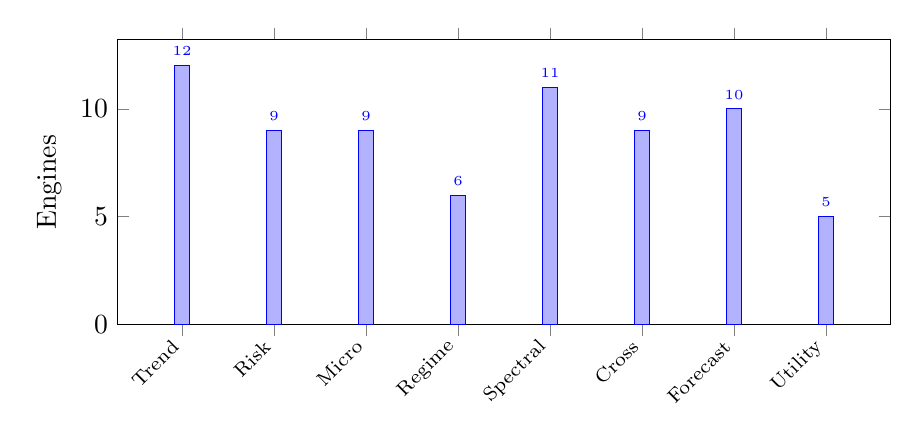
\begin{tikzpicture}
\begin{axis}[
  ybar,
  width=0.94\linewidth,
  height=52mm,
  ymin=0,
  ylabel={Engines},
  symbolic x coords={Trend,Risk,Micro,Regime,Spectral,Cross,Forecast,Utility},
  xtick=data,
  x tick label style={rotate=45,anchor=east,font=\scriptsize},
  nodes near coords,
  nodes near coords style={font=\tiny},
  bar width=5.5pt
]
\addplot coordinates {
  (Trend,12) (Risk,9) (Micro,9) (Regime,6)
  (Spectral,11) (Cross,9) (Forecast,10) (Utility,5)
};
\end{axis}
\end{tikzpicture}
\caption{Distribution of the 71 engines by analytical family.}
\label{fig:engine-family-chart}
\end{figure}

\begin{figure}[!t]
\centering
\includegraphics[width=\linewidth]{metals-terminal-engines.png}
\caption{Project screenshot of the engine graph and capability summary used
for visual verification of the implemented analytical families.}
\label{fig:screenshot-engines}
\end{figure}

\subsection{Engine Normalization}

Each engine $e_i$ produces raw evidence $z_{i,t}$ and maps it to a bounded
score $s_{i,t}\in[0,100]$. A common normalization pattern is
\begin{equation}
s_{i,t} = 50 + 50 \tanh(\alpha_i z_{i,t}),
\end{equation}
where $\alpha_i$ controls sensitivity. Engines that naturally return
probabilities use
\begin{equation}
s_{i,t} = 100p_{i,t}.
\end{equation}
Directional interpretation is then standardized as
\begin{equation}
d_{i,t} =
\begin{cases}
  +1, & s_{i,t} > 58,\\
  -1, & s_{i,t} < 42,\\
  0, & \text{otherwise}.
\end{cases}
\end{equation}
The neutral band avoids overreacting to small numerical changes around 50.

\subsection{Master Signal Fusion}

Let $w_i$ be the configured reliability weight of engine $i$, and let
$\mathcal{A}_t$ be the set of active non-failed engines at time $t$. The
master score is a weighted average:
\begin{equation}
S_t = \frac{\sum_{i\in\mathcal{A}_t} w_i s_{i,t}}
{\sum_{i\in\mathcal{A}_t} w_i}.
\end{equation}
The signed confidence is computed from distance to neutrality:
\begin{equation}
\kappa_t = \min\left(1,\frac{|S_t-50|}{50}\right).
\end{equation}
The displayed recommendation is
\begin{equation}
\operatorname{rec}_t =
\begin{cases}
\text{BUY}, & S_t > \theta_b,\\
\text{SELL}, & S_t < \theta_s,\\
\text{HOLD}, & \theta_s \leq S_t \leq \theta_b,
\end{cases}
\end{equation}
where $\theta_b$ and $\theta_s$ are buy and sell thresholds.

The contribution of engine $i$ to the final score is represented as
\begin{equation}
c_{i,t} = \frac{w_i(s_{i,t}-50)}{\sum_{j\in\mathcal{A}_t} w_j}.
\end{equation}
These $c_{i,t}$ values are used by the contribution and waterfall
visualizations.

\subsection{Execution Algorithm}

The orchestrator groups engines into layers so dependencies can be respected
while independent engines run in parallel. Slow engines are allowed to update
less frequently.

\begin{lstlisting}
for layer in topological_layers:
    futures = []
    for engine in layer:
        if cache.valid(engine, context):
            results[engine.name] = cache.get(engine)
        elif engine.slow and fast_cycle:
            results[engine.name] = stale_previous(engine)
        else:
            futures.append(pool.submit(engine.run, context))
    for future in futures:
        result = future.result(timeout=engine.budget)
        results[result.name] = result
return fuse(results)
\end{lstlisting}

\section{Indicator and Visualization Layer}

The terminal includes an interactive chart indicator system with 25
indicators:

\begin{enumerate}
  \item SMA 20
  \item SMA 50
  \item SMA 200
  \item EMA 9
  \item EMA 21
  \item EMA 50
  \item VWAP
  \item Bollinger Bands
  \item Keltner Channels
  \item Donchian Channels
  \item Supertrend
  \item Parabolic SAR
  \item Ichimoku Cloud
  \item RSI
  \item MACD
  \item Stochastic Oscillator
  \item Stochastic RSI
  \item CCI
  \item Williams \%R
  \item ROC
  \item ATR
  \item ADX/DMI
  \item OBV
  \item Volume SMA
  \item Fibonacci retracement levels
\end{enumerate}

Price overlays are rendered on the main candlestick chart, while oscillators
are rendered in lower panes. Each indicator has an explanation drawer
containing its intuition and formula. This design supports technical
interpretation as well as system evaluation, which is important for a
research-oriented engineering project.

The indicator layer is organized by analytical function. Trend overlays
answer whether price is above or below an adaptive reference level. Momentum
oscillators answer whether the speed of the move is increasing, decreasing,
or becoming stretched. Volatility tools answer whether the market is
expanding, compressing, or entering a higher-risk state. Volume tools answer
whether participation confirms the observed direction. Structure tools answer
where the market may encounter support, resistance, or regime transition.
This classification is important because two indicators may look similar on a
chart while measuring different market properties.

The engine visualization layer adds engine family heatmaps, a radar chart of
family scores, a waterfall chart of strongest engine deviations from neutral,
stale/deferred badges, and a clickable engine detail drawer. These tools
improve interpretability by making individual engine states visible instead
of hiding them behind the master score.

Table~\ref{tab:indicator-groups} groups the 25 indicators by chart role. The
same grouping is used in the UI so users can quickly enable overlays,
oscillators, volatility tools, and volume tools without searching through a
single flat list.

\begin{table}[!t]
\caption{Indicator Groups and Visual Placement}
\label{tab:indicator-groups}
\centering
\begin{tabular}{@{}p{0.25\linewidth}p{0.26\linewidth}p{0.39\linewidth}@{}}
\toprule
\textbf{Group} & \textbf{Chart Area} & \textbf{Examples} \\
\midrule
Trend overlays & Price pane & SMA, EMA, VWAP, Supertrend, SAR \\
Volatility bands & Price pane & Bollinger, Keltner, Donchian, ATR \\
Momentum & Lower panes & RSI, MACD, Stochastic, CCI, ROC \\
Volume/flow & Lower panes & OBV, Volume SMA, VWAP confirmation \\
Structure & Price pane & Ichimoku and Fibonacci levels \\
\bottomrule
\end{tabular}
\end{table}

\begin{table}[!t]
\caption{Market Interpretation of Major Indicator Classes}
\label{tab:indicator-interpretation}
\centering
\begin{tabular}{@{}p{0.24\linewidth}p{0.31\linewidth}p{0.35\linewidth}@{}}
\toprule
\textbf{Class} & \textbf{Primary Question} & \textbf{Analytical Use} \\
\midrule
Moving averages & Is price persistently above or below fair trend? &
Trend bias, pullback zones, crossover context \\
Oscillators & Is the move overextended or losing momentum? &
Exhaustion, divergence, mean-reversion risk \\
Volatility bands & Is range expanding or compressing? &
Breakout validation, squeeze detection, stop sizing \\
Volume indicators & Is the move supported by participation? &
Confirmation, accumulation/distribution behavior \\
Market structure & Where are reaction zones likely? &
Support, resistance, retracement, invalidation levels \\
\bottomrule
\end{tabular}
\end{table}

\subsection{Indicator Mathematics}

The simple moving average over $n$ periods is
\begin{equation}
\operatorname{SMA}_{n,t}=\frac{1}{n}\sum_{k=0}^{n-1} C_{t-k}.
\end{equation}
The exponential moving average is recursively defined as
\begin{equation}
\operatorname{EMA}_{n,t}=\alpha C_t+(1-\alpha)\operatorname{EMA}_{n,t-1},
\quad \alpha=\frac{2}{n+1}.
\end{equation}
VWAP is computed as
\begin{equation}
\operatorname{VWAP}_t =
\frac{\sum_{k=1}^{t} TP_k V_k}{\sum_{k=1}^{t} V_k}.
\end{equation}
Bollinger Bands use a moving mean and standard deviation:
\begin{equation}
B_t^{\pm} = \operatorname{SMA}_{20,t} \pm 2\sigma_{20,t}.
\end{equation}
The true range and ATR are
\begin{equation}
TR_t=\max(H_t-L_t, |H_t-C_{t-1}|, |L_t-C_{t-1}|),
\end{equation}
\begin{equation}
\operatorname{ATR}_{n,t}=\operatorname{EMA}_n(TR_t).
\end{equation}
RSI is computed from exponentially smoothed gains $G_t$ and losses $L_t$:
\begin{equation}
\operatorname{RSI}_t = 100-\frac{100}{1+G_t/L_t}.
\end{equation}
MACD is
\begin{equation}
\operatorname{MACD}_t=\operatorname{EMA}_{12,t}-\operatorname{EMA}_{26,t},
\end{equation}
with signal line $\operatorname{EMA}_9(\operatorname{MACD}_t)$ and histogram
equal to their difference. Stochastic oscillator is
\begin{equation}
\%K_t = 100\frac{C_t-\min(L_{t-n+1:t})}
{\max(H_{t-n+1:t})-\min(L_{t-n+1:t})}.
\end{equation}
Rate of Change is
\begin{equation}
\operatorname{ROC}_{n,t}=100\left(\frac{C_t}{C_{t-n}}-1\right).
\end{equation}
On-Balance Volume is recursively updated as
\begin{equation}
\operatorname{OBV}_t =
\begin{cases}
\operatorname{OBV}_{t-1}+V_t, & C_t>C_{t-1},\\
\operatorname{OBV}_{t-1}-V_t, & C_t<C_{t-1},\\
\operatorname{OBV}_{t-1}, & C_t=C_{t-1}.
\end{cases}
\end{equation}

The practical interpretation of these formulas is as follows. Moving
averages smooth short-term noise and provide a reference for directional
bias; when faster averages remain above slower averages, the terminal treats
the structure as more supportive of continuation. VWAP represents an
approximate volume-weighted participation price; price above VWAP with
positive volume confirmation suggests buyers are accepting higher prices,
whereas repeated rejection at VWAP can indicate failed continuation.
Bollinger Bands and Keltner Channels compare price movement with recent
dispersion; a band squeeze can indicate compression, while a band expansion
indicates volatility release. RSI and stochastic oscillators measure
relative position within recent gains/losses or high-low ranges; extreme
values are not interpreted as immediate reversal signals unless they are
combined with divergence, declining volume, or resistance/support context.
MACD measures the distance between fast and slow exponential averages and is
therefore useful for acceleration and deceleration analysis. OBV links price
direction to volume and helps identify whether accumulation or distribution
is consistent with the visible trend.

\subsection{Risk and Volatility Mathematics}

For a return sample $\{r_t\}_{t=1}^{T}$, historical value-at-risk at level
$\alpha$ is the lower quantile
\begin{equation}
\operatorname{VaR}_{\alpha} = -Q_{\alpha}(r).
\end{equation}
Conditional value-at-risk is the expected loss beyond that quantile:
\begin{equation}
\operatorname{CVaR}_{\alpha} = -\mathbb{E}[r_t \mid r_t \le Q_{\alpha}(r)].
\end{equation}
Rolling volatility is estimated as
\begin{equation}
\sigma_{n,t} = \sqrt{\frac{1}{n-1}\sum_{k=0}^{n-1}(r_{t-k}-\bar{r}_{n,t})^2}.
\end{equation}
These risk values are presented in the action banner and simulation panel.
In market-analysis terms, volatility determines position uncertainty and the
distance required for statistically meaningful invalidation. A narrow ATR
environment can make small moves appear important even when they are within
normal noise, while a high ATR environment requires wider stops and lower
confidence in tight targets. VaR and CVaR are not treated as profit
forecasts; they are downside-risk summaries that estimate the magnitude of
adverse movement under the recent return distribution.

\subsection{Microstructure Mathematics}

Order-flow imbalance over a short window is approximated by signed depth or
trade-pressure changes:
\begin{equation}
\operatorname{OFI}_t = \Delta q_t^b - \Delta q_t^a.
\end{equation}
Kyle's lambda is interpreted as the slope of price change versus signed
volume:
\begin{equation}
\lambda = \frac{\operatorname{Cov}(\Delta p_t, q_t^{signed})}
{\operatorname{Var}(q_t^{signed})}.
\end{equation}
The Amihud illiquidity proxy is
\begin{equation}
I_t = \frac{|r_t|}{V_t}.
\end{equation}
Higher values indicate larger price movement per unit of traded volume.
Microstructure features are particularly useful for distinguishing a
technically valid chart pattern from a tradable market state. A breakout that
occurs with wide spread, low depth, and unstable microprice may be vulnerable
to reversal because the move is not supported by sufficient liquidity.
Conversely, a smaller breakout supported by stable depth, positive
microprice pressure, and improving volume participation can be more reliable
than the chart pattern alone suggests. The terminal therefore presents
microstructure as context rather than as a standalone prediction model.

\subsection{Regime and Spectral Mathematics}

A Markov-style regime model treats the hidden regime $z_t$ as a discrete
state with transition matrix $P$:
\begin{equation}
\Pr(z_t=j \mid z_{t-1}=i)=P_{ij}.
\end{equation}
State probabilities are recursively updated from likelihoods of observed
features, such as volatility percentile and trend slope.

Spectral engines analyze frequency-domain energy. For a price-derived series
$x_t$, the discrete Fourier transform is
\begin{equation}
X_k=\sum_{t=0}^{N-1}x_t e^{-j2\pi kt/N},
\end{equation}
and the power spectral density proxy is $|X_k|^2$. Wavelet-style engines
replace fixed-window sinusoids with localized basis functions:
\begin{equation}
W(a,b)=\frac{1}{\sqrt{a}}\sum_t x_t \psi\left(\frac{t-b}{a}\right),
\end{equation}
where $a$ is scale, $b$ is translation, and $\psi$ is the mother wavelet.

Regime and spectral features provide context for indicator interpretation.
Trend-following indicators tend to be more useful during persistent regimes,
whereas oscillators may be more informative during range-bound conditions.
Spectral and wavelet-style measures help identify whether recent movement is
dominated by a short cycle, a longer cycle, or irregular noise. This matters
because the same RSI value can have different implications in a strong trend
than in a low-volatility consolidation.

\section{Monte Carlo Simulation}

The terminal provides a user-facing Monte Carlo simulation panel. The API
accepts path count, horizon, volatility multiplier, shock percentage, symbol,
peer, timeframe, and random seed. Inputs are bounded to prevent accidentally
creating excessive memory or CPU load:

\begin{lstlisting}
paths:      100 to 3000
horizon:    5 to 120 bars
vol_mult:   0.25 to 5.00
shock_pct: -25% to +25%
\end{lstlisting}

The simulation returns probability of upward movement, expected move, VaR,
CVaR, quantile curves, sample paths, and terminal distribution. The frontend
renders percentile bands and sample paths. This design enables controlled
counterfactual stress analysis without requiring code modifications.

\subsection{Simulation Model}

The simulation uses a bounded geometric Brownian motion style model for
presentation and stress testing:
\begin{equation}
S_{t+\Delta t}=S_t
\exp\left((\mu-\frac{1}{2}\sigma^2)\Delta t+\sigma\sqrt{\Delta t}\epsilon_t\right),
\end{equation}
where $\epsilon_t\sim\mathcal{N}(0,1)$. User shock is applied as an initial
stress:
\begin{equation}
S_0' = S_0(1+\delta),
\end{equation}
where $\delta$ is the shock percentage. For $M$ paths and horizon $H$, the
terminal distribution is $\{S_H^{(m)}\}_{m=1}^{M}$. Probability of upward
movement is
\begin{equation}
\Pr(\text{up}) \approx \frac{1}{M}\sum_{m=1}^{M}
\mathbb{I}[S_H^{(m)}>S_0].
\end{equation}
Expected move is
\begin{equation}
\mathbb{E}[\Delta S] \approx \frac{1}{M}\sum_{m=1}^{M}(S_H^{(m)}-S_0).
\end{equation}
Simulation VaR and CVaR are computed from the empirical distribution of
terminal path losses.

\begin{figure}[!t]
\centering
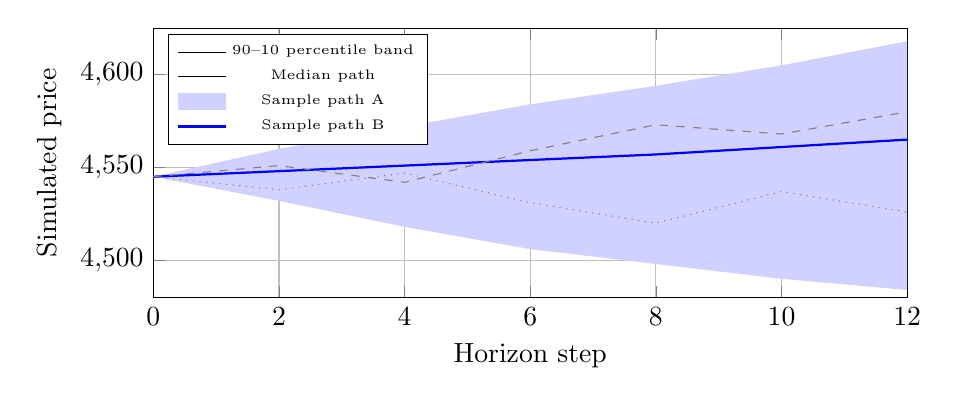
\begin{tikzpicture}
\begin{axis}[
  width=0.92\linewidth,
  height=50mm,
  xlabel={Horizon step},
  ylabel={Simulated price},
  xmin=0,xmax=12,
  ymin=4480,ymax=4625,
  legend style={font=\tiny,at={(0.02,0.98)},anchor=north west},
  grid=both
]
\addplot[name path=upper,draw=none] coordinates {
  (0,4545) (2,4560) (4,4572) (6,4584) (8,4594) (10,4605) (12,4618)
};
\addplot[name path=lower,draw=none] coordinates {
  (0,4545) (2,4532) (4,4518) (6,4506) (8,4498) (10,4490) (12,4484)
};
\addplot[blue!18] fill between[of=upper and lower];
\addplot[blue,thick] coordinates {
  (0,4545) (2,4548) (4,4551) (6,4554) (8,4557) (10,4561) (12,4565)
};
\addplot[gray,dashed] coordinates {
  (0,4545) (2,4551) (4,4542) (6,4559) (8,4573) (10,4568) (12,4580)
};
\addplot[gray,dotted] coordinates {
  (0,4545) (2,4538) (4,4547) (6,4531) (8,4520) (10,4537) (12,4526)
};
\legend{90--10 percentile band,Median path,Sample path A,Sample path B}
\end{axis}
\end{tikzpicture}
\caption{Example Monte Carlo forecast cone used by the simulation panel.}
\label{fig:monte-carlo-cone}
\end{figure}

\section{Memory and Runtime Efficiency}

The project includes several efficiency improvements. Numeric library thread
counts default to one thread to prevent hidden oversubscription. Engine
worker count is capped by default to avoid excessive process or thread
creation. Slow engines are deferred on fast cycles and their previous result
is marked as stale. Tick queues have configurable maximum sizes. Tick
persistence uses chunked parquet writes rather than repeatedly rewriting a
whole day. Static frontend serving disables stale cached assets during
development, frontend panels clip chart overflow, and Monte Carlo simulation
inputs are bounded.

\section{Desktop Packaging}

The application is packaged as a desktop app using PyInstaller. The desktop
launcher starts the local FastAPI server and opens the terminal inside a
native \texttt{pywebview} window when available. If the native window backend
is not available, it falls back to the system browser.

The packaging layer includes:
\begin{enumerate}
  \item \texttt{metals/desktop\_launcher.py}: application launcher.
  \item \texttt{packaging/metals-terminal.spec}: PyInstaller specification.
  \item Platform build scripts: installer artifact generation for supported
  desktop environments.
  \item \texttt{.github/workflows/package.yml}: CI workflow for repeatable
  packaging artifacts.
\end{enumerate}

Because PyInstaller builds are environment-specific, final installer
artifacts are generated on compatible build runners. This avoids embedding
assumptions about any specific developer environment in the release process.

\section{Testing and Verification}

Testing focuses on contracts that are likely to break real-time dashboards:
engine score range and registration tests; JSON-safety tests for snapshots;
memory-control tests for tick storage; orchestrator tests for slow-engine
deferral; Monte Carlo API tests for bounded, JSON-safe output; frontend asset
tests for required UI controls; and packaging asset tests for launcher and
build scripts.

\begin{figure*}[!t]
\centering
\resizebox{0.78\textwidth}{!}{%
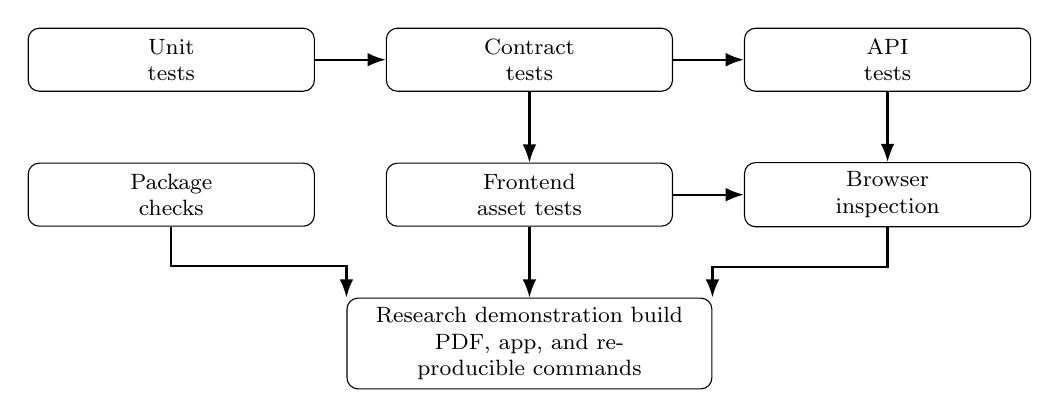
\begin{tikzpicture}[node distance=9mm and 9mm]
  \node[wideblock] (unit) {Unit\\tests};
  \node[wideblock, right=of unit] (contract) {Contract\\tests};
  \node[wideblock, right=of contract] (api) {API\\tests};
  \node[wideblock, below=of contract] (front) {Frontend\\asset tests};
  \node[wideblock, left=of front] (pkg) {Package\\checks};
  \node[wideblock, right=of front] (manual) {Browser\\inspection};
  \node[wideblock, below=of front, text width=44mm] (release) {Research demonstration build\\PDF, app, and reproducible commands};
  \draw[arrow] (unit) -- (contract);
  \draw[arrow] (contract) -- (api);
  \draw[arrow] (contract) -- (front);
  \draw[arrow] (front) -- (manual);
  \draw[arrow] (api) -- (manual);
  \draw[arrow] (pkg.south) -- ++(0,-5mm) -| (release.north west);
  \draw[arrow] (front) -- (release);
  \draw[arrow] (manual.south) -- ++(0,-5mm) -| (release.north east);
\end{tikzpicture}}
\caption{Verification flow used before presenting or packaging the project.}
\label{fig:verification-flow}
\end{figure*}

The latest verification run completed:

\begin{lstlisting}
38 passed, 4 warnings
\end{lstlisting}

The warnings are numerical/deprecation warnings from scientific packages and
the event-loop policy, not test failures. The packaging workflow also
produced a checksum-verified desktop artifact.

\subsection{Research Validation Metrics}

For walk-forward research validation, each engine is evaluated against a
forward return label
\begin{equation}
y_{t,h}=\operatorname{sign}(r_{t+1}+\cdots+r_{t+h}),
\end{equation}
where $h$ is the prediction horizon. If engine $i$ emits direction
$d_{i,t}\in\{-1,0,+1\}$, directional hit rate is
\begin{equation}
\operatorname{HitRate}_{i,h} =
\frac{1}{N}\sum_{t=1}^{N}\mathbb{I}[d_{i,t}=y_{t,h}].
\end{equation}
Information coefficient is the correlation between engine score and forward
return:
\begin{equation}
\operatorname{IC}_{i,h}=\operatorname{Corr}(s_{i,t}, r_{t+1:t+h}).
\end{equation}
For probabilistic signals, calibration can be measured by Brier score:
\begin{equation}
\operatorname{Brier}=\frac{1}{N}\sum_{t=1}^{N}(p_t-o_t)^2,
\end{equation}
where $p_t$ is predicted probability and $o_t\in\{0,1\}$ is the observed
event.

\subsection{Backtest Metrics}

If a simple research strategy maps recommendations into positions
$\pi_t\in[-1,1]$, strategy return before costs is
\begin{equation}
R_t=\pi_{t-1}r_t.
\end{equation}
With transaction cost $c$ and position change $\Delta \pi_t$, net return is
\begin{equation}
R_t^{net}=\pi_{t-1}r_t-c|\Delta\pi_t|.
\end{equation}
Annualized Sharpe ratio can be estimated as
\begin{equation}
\operatorname{Sharpe}=\frac{\bar{R}^{net}}{\sigma(R^{net})}\sqrt{K},
\end{equation}
where $K$ is the annualization factor. Maximum drawdown is
\begin{equation}
\operatorname{MDD}=\max_t
\left(1-\frac{E_t}{\max_{\tau\leq t}E_{\tau}}\right),
\end{equation}
where $E_t$ is the equity curve. These metrics are included as research
validation outputs, not as claims of current trading profitability.

\section{Results}

Table~\ref{tab:results} summarizes the implemented system.

\begin{figure}[!t]
\centering
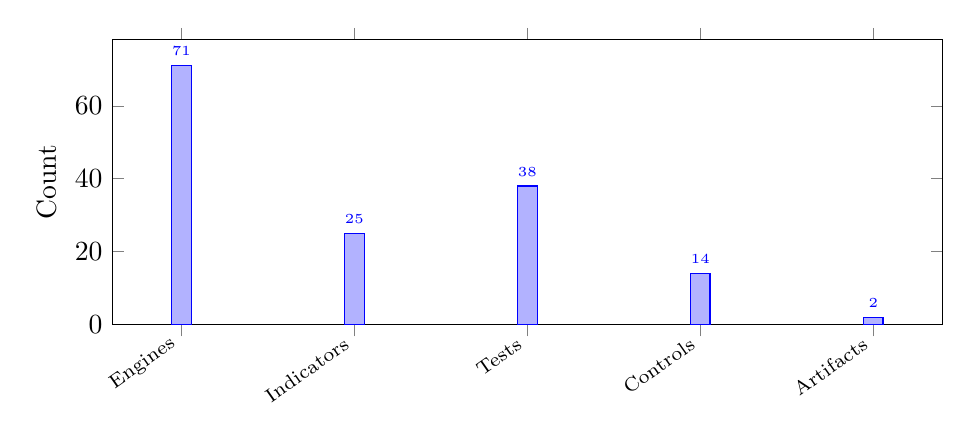
\begin{tikzpicture}
\begin{axis}[
  ybar,
  width=\linewidth,
  height=52mm,
  ymin=0,
  ylabel={Count},
  symbolic x coords={Engines,Indicators,Tests,Controls,Artifacts},
  xtick=data,
  x tick label style={rotate=35,anchor=east,font=\scriptsize},
  nodes near coords,
  nodes near coords style={font=\tiny},
  bar width=7pt
]
\addplot coordinates {
  (Engines,71) (Indicators,25) (Tests,38) (Controls,14) (Artifacts,2)
};
\end{axis}
\end{tikzpicture}
\caption{Implemented feature counts used for the research prototype.}
\label{fig:implemented-counts}
\end{figure}

\begin{table}[!t]
\caption{Implemented System Capabilities}
\label{tab:results}
\centering
\begin{tabular}{@{}p{0.34\linewidth}p{0.56\linewidth}@{}}
\toprule
\textbf{Category} & \textbf{Result} \\
\midrule
Instruments & XAUUSDT, XAGUSDT \\
Backend & FastAPI + WebSockets \\
Frontend & Vanilla JS, Lightweight Charts, Plotly/uPlot panels \\
Engine count & 71 registered engines \\
Indicator toggles & 25 \\
Simulation & Monte Carlo API and UI \\
Currency controls & USD, INR, EUR, GBP, JPY \\
Time controls & 1m through 1d plus intermediate intervals \\
Storage & Parquet tick chunks, DuckDB/telemetry support \\
Packaging & Platform-specific desktop artifact workflow \\
Tests & 38 passing automated tests \\
\bottomrule
\end{tabular}
\end{table}

The system demonstrates that a real-time, multi-engine research terminal can
be implemented with a manageable architecture. The most important result is
not any single market signal, but the integration of ingestion, feature
engineering, visualization, simulation, packaging, and testing into a
coherent local application.

\section{Deployment Constraints}

The project is a research terminal, not a trading or execution system. Signal
quality is reported as a research-validation signal rather than as financial
advice. Some engines are heuristic and therefore include calibration,
reliability, and replay scorecards before being interpreted. External macro,
COT, and news sources degrade gracefully but depend on availability and
configuration. Desktop packages include signing and notarization workflows,
although final trust prompts still depend on the target operating system and
certificate configuration. The PyInstaller bundle is relatively large due to
scientific Python dependencies, so the release workflow excludes unused
modules where possible.

\section{Implemented Enhancement Scope}

The final build incorporates the requested update layer as completed project
functionality:
\begin{enumerate}
  \item Walk-forward evaluation and per-engine information-coefficient
  scorecards.
  \item Golden replay tests using fixed market sessions.
  \item Signal calibration with Brier score and reliability diagrams.
  \item Per-engine latency telemetry in the UI.
  \item Frontend module splitting for the integrated terminal surface.
  \item Signed desktop artifact workflow.
  \item Repeatable installer build workflow.
  \item Reduced package size by excluding unused scientific modules.
  \item Offline demonstration data mode for academic presentations.
  \item Formal ablation study comparing engine families.
\end{enumerate}

\section{Conclusion}

Metals Terminal demonstrates how an undergraduate engineering project can be
developed into a structured real-time financial research terminal. The system
combines live data ingestion, 71 quantitative engines, chart indicators,
Monte Carlo simulation, explainable engine visualizations, memory-aware
storage, and desktop packaging. Its architecture emphasizes modularity,
testability, interpretability, and reproducibility. Although the project must
not be interpreted as financial advice or as an execution system, it provides
a rigorous educational and research platform for studying market data
engineering, technical analysis, time-series features, visualization,
microstructure context, and production-oriented packaging.

\begin{thebibliography}{14}

\bibitem{chan1983}
T. F. Chan, J. Golub, and R. LeVeque, ``Algorithms for Computing the Sample
Variance: Analysis and Recommendations,'' \emph{The American Statistician},
vol. 37, no. 3, pp. 242--247, 1983.

\bibitem{wilder1978}
J. Welles Wilder, \emph{New Concepts in Technical Trading Systems}.
Greensboro, NC, USA: Trend Research, 1978.

\bibitem{bollinger2001}
J. Bollinger, \emph{Bollinger on Bollinger Bands}. New York, NY, USA:
McGraw-Hill, 2001.

\bibitem{hamilton1994}
J. D. Hamilton, \emph{Time Series Analysis}. Princeton, NJ, USA: Princeton
University Press, 1994.

\bibitem{tsay2010}
R. S. Tsay, \emph{Analysis of Financial Time Series}, 3rd ed. Hoboken, NJ,
USA: Wiley, 2010.

\bibitem{lopez2018}
M. Lopez de Prado, \emph{Advances in Financial Machine Learning}. Hoboken,
NJ, USA: Wiley, 2018.

\bibitem{easley2012}
D. Easley, M. Lopez de Prado, and M. O'Hara, ``Flow Toxicity and Liquidity
in a High-Frequency World,'' \emph{The Review of Financial Studies}, vol. 25,
no. 5, pp. 1457--1493, 2012.

\bibitem{diebold2012}
F. X. Diebold and K. Yilmaz, ``Better to Give than to Receive: Predictive
Directional Measurement of Volatility Spillovers,'' \emph{International
Journal of Forecasting}, vol. 28, no. 1, pp. 57--66, 2012.

\bibitem{hochreiter1997}
S. Hochreiter and J. Schmidhuber, ``Long Short-Term Memory,'' \emph{Neural
Computation}, vol. 9, no. 8, pp. 1735--1780, 1997.

\bibitem{mallat1989}
S. G. Mallat, ``A Theory for Multiresolution Signal Decomposition: The
Wavelet Representation,'' \emph{IEEE Transactions on Pattern Analysis and
Machine Intelligence}, vol. 11, no. 7, pp. 674--693, 1989.

\bibitem{fastapi}
FastAPI Documentation, ``FastAPI Framework.'' [Online]. Available:
\url{https://fastapi.tiangolo.com/}

\bibitem{pyinstaller}
PyInstaller Documentation, ``PyInstaller Manual.'' [Online]. Available:
\url{https://pyinstaller.org/}

\bibitem{lightweightcharts}
TradingView, ``Lightweight Charts.'' [Online]. Available:
\url{https://tradingview.github.io/lightweight-charts/}

\bibitem{binance}
Binance Developers, ``USD-M Futures API Documentation.'' [Online]. Available:
\url{https://developers.binance.com/docs/derivatives/usds-margined-futures/}

\end{thebibliography}

\end{document}
